\documentclass{article}

%%%%%%%%%%%%%%% LIBRERIAS %%%%%%%%%%%%%%%%%%%%%
\usepackage[thinc]{esdiff}
\usepackage{amsmath}
\usepackage{caption}
\usepackage{physics}
\usepackage{titlesec}
\usepackage{titletoc}
\usepackage{graphicx}
\usepackage[spanish,es-tabla]{babel} % 'es-tabla' cambia Cuadro→Tabla
\usepackage{hyperref}                % cargar después de babel
\usepackage{float}
\usepackage{circuitikz}
\usepackage[left=3cm,right=3cm]{geometry} %para margenes
\usepackage{subfiles} 
\usepackage{subcaption}
\usepackage{pgfplots}
\pgfplotsset{compat=1.18}
\usepackage{booktabs} % Para tablas con tematica de paper cientifico
\usepackage{siunitx}  % Para alinear números en las tablas d:
\usepackage[backend=biber, style=ieee]{biblatex} % referencias
\addbibresource{sample.bib} %archivo con referencias

%%%%%%%%%%%%%%%%%%% VARIABLES %%%%%%%%%%%%%%%%%%%%
\newcommand{\Facultad}{Instituto Tecnológico \\de\\ Buenos Aires} %constantes
\newcommand{\TPn}{Trabajo Práctico N°3: Principios de Motores}
\newcommand{\TPtema}{}
\renewcommand{\thesection}{\arabic{section}}          % 2
\renewcommand{\thesubsection}{\quad \alph{subsection}}   % a
\renewcommand{\thesubsubsection}{\quad \thesubsection.~\roman{subsubsection}} % a. i
\graphicspath{{imagenes/}} %para que acceda a las fotos en la carpeta directamente


%%%%%%%%%%%%%%%%%% FORMATO TÍTULO Y NUMERACIÓN %%%%%%%%%%%%%%%%%%%
% Numeración de secciones
\renewcommand{\thesection}{\arabic{section}.}          
\renewcommand{\thesubsection}{\thesection\arabic{subsection}}       
\renewcommand{\thesubsubsection}{$\alph{subsubsection}$}

% Numerar hasta subsubsecciones
\setcounter{secnumdepth}{3}

% Formato de títulos
\titleformat{\section}{\Large\bfseries}{\thesection}{1em}{}
\titleformat{\subsection}{\large\bfseries}{\thesubsection}{0.5em}{}
\titleformat{\subsubsection}{\normalsize\bfseries}{\thesubsubsection}{0.5em}{}

\begin{document}

\begin{titlepage} %creo portada

        \begin{flushleft}
            \centering
            
\includegraphics[width=0.3\textwidth]{Logo_ITBA.png}
        \end{flushleft}

        \centering
            
        {\scshape\LARGE \Facultad \par} %\par sirve para indicar un final de parrafo
        \vspace{1cm}                    %esto hace un espacio entre lineas de 1cm


        {\huge\bfseries \TPn \par}
        \vspace{1cm}
        {\Large Tecnología de Materiales Electrónicos\\ 25.12 \par}
        \vspace{0.5cm}
        %{\Large \TPtema \par}
        %\vfill                      %sirve para rellenar el espacio y quede simétrico.
        {\Large \textbf{ Informe} \par}
        \vspace{0.5cm}
         {\Large Grupo 2 \par}
        \vspace{2cm}
        {\large Juan Bautista Correa Uranga \hfill Legajo: 65016 \par} 
        {\large Juan Ignacio Caorsi \hfill Legajo: 65532  \par}
        {\large Rita Moschini \hfill Legajo: 67026 \par} 
        {\large Lucas Solar Grillo \hfill Legajo: 63322\par}
        \vfill
        {\large \today\par}
        \vfill

\end{titlepage}

\section{Resumen}

Este trabajo práctico tiene como objetivo construir un motor de continua rudimentario basado en los principios físicos estudiados con anterioridad.

\section{Desarrollo}

Los materiales utilizados fueron
\begin{itemize}
	\item \href{https://www.bto.pl/pdf/10681/MAX-EU-D_eng_tds.pdf}{Batería tipo D de 1,5 V de Energizer Max}
	\item Cable de cobre de 0,2 mm
	\item Imán permanente de neodimio
	\item Clips de papel
	\item Cable de cobre de 0,6 mm
	\item Base de cartón
	\item Cinta de papel
\end{itemize}

Doblando alambres como se observa en la figura \ref{fotoMotor}, se realizó un soporte mecánico para sostener al motor dc diseñado.

\begin{figure}[H]
\centering
   	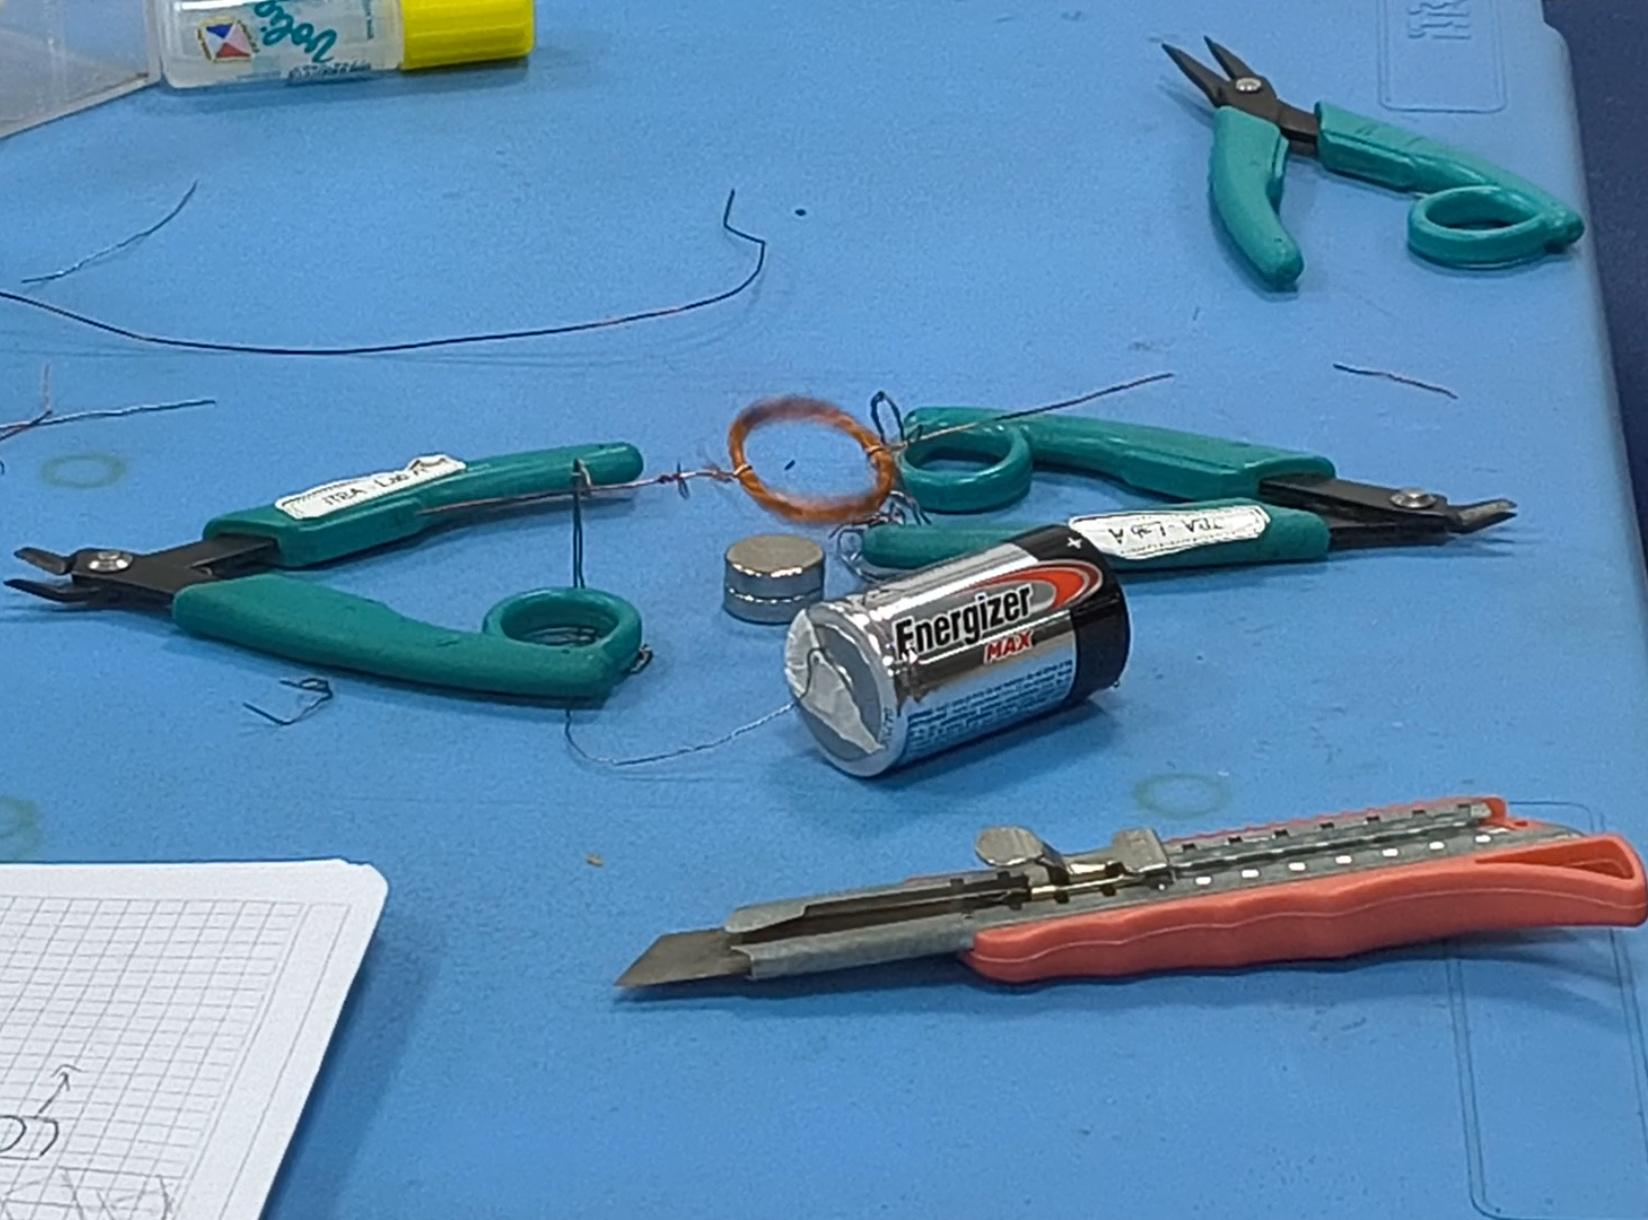
\includegraphics[width=0.5\textwidth]{fotoMotor.png}
    \caption{Motor DC.}
    \label{fotoMotor}
\end{figure}

\section{Diseño del rotor}
El motor DC diseñado consiste en una espira circular de cobre, colocada sobre un iman permanente de neodimio
 y conectada a una batería de 1,5 V. Dado que la  \href{https://www.bto.pl/pdf/10681/MAX-EU-D_eng_tds.pdf}{hoja de datos de la batería} 
 incluye un gráfico de corriente de 0 a 1 A, tomamos como corriente máxima 500 mA. Así, obtuvimos
\begin{equation*}
    R = \frac{1,5 \, V}{500 \, mA} = 3 \, \Omega
\end{equation*}
Dado que se busca que la corriente sea menor o igual que 500 mA para no exigirle a la batería más corriente
 de la que pudiera entregar, esos $ 3 \, \Omega $ son realmente una cota inferior. Luego, se utilizó la ecuación
\begin{equation*}
    R = \frac{\rho_{Cu} \cdot L_{total}}{A_{cable}}
\end{equation*}
donde $\rho_{Cu}=1,72\cdot 10^{-8} \, \Omega\cdot m$ es la resistividad del cobre, $L_{total}$ es la longitud
total de la espira de cobre y $A_{cable}$ es el área transversal del cable de cobre. Dado que se buscó la 
mayor resistencia posible para minimizar la corriente, se buscó a su vez minizimar el área, por lo que se 
utilizó el cable menor diámetro disponible en el pañol, es decir de 0,2 mm. Así, la longitud que requeríamos
resultó ser 
\begin{align*}
    L_{total} &=\frac{R \cdot A_{cable}}{\rho_{Cu}} \\
              &= \frac{R \cdot \pi \left( \frac{d}{2} \right)^2}{\rho_{Cu}} \\
              &= 5,48 \, m
\end{align*}
A fines prácticos, dado que el valor tomado de R realmente es una cota inferior, y R es directamente 
proporcional a $L_{total}$, se tomó $L_{total} = 6 \, m$.
\par Luego, se buscó que la espira tuviera un diámetro ligeramente mayor al de los imanes, y finalmente se 
decidió en un diámetro de 30 mm. Así, el perímetro de la misma resultó ser
$perimetroEspira \, = \, \pi \cdot 30\cdot 10^{-3} \, m = 94,25 mm$ y así $\frac{L_{total}}{perimetroEspira} \geq N$
donde N es la cantidad de vueltas de la espira, y reemplazando, resulta que $63,66 \geq N$. Debido a error
humano, la cantidad de vueltas finalmente resultó ser N=60.

\section{Diseño del colector}
 Para mantener el giro del motor en un único sentido, es indispensable la acción del colector. En este
 prototipo, se implementa quitando el esmalte aislante de los extremos del bobinado de manera asimétrica 
 (raspando solo la mitad de la circunferencia). Su función principal es actuar como conmutación mecánica:
 permite el paso de corriente solo durante media vuelta del rotor (idealmente 180◦). En esta fase, el torque
 generado empuja a la bobina, dándole aceleración angular. Durante la otra media vuelta, el barniz intacto 
 interrumpe el circuito. Al no haber corriente, no se produce fuerza magnética en sentido opuesto que frene
 la rotación, permitiendo que la bobina complete la revolución por inercia.

\section{Campo magnético}
Al circular corriente por la bobina, esta genera su propio campo magnético. Asumiendo que la bobina es 
plana y circular, se puede obtener mediante la Ley de Biot-Savart
\begin{equation*}
    B_{autoinducido}=\frac{\mu_0 \cdot N \cdot I}{D}
\end{equation*}
donde D es el diámetro de la espira, 30 mm. Tomando $\mu_0=4\pi \cdot 10^{-7}$, resulta que
$B_{autoinducido}=1,25 \, mT$. Luego, para estimar la magnitud del campo magnético generado por los imanes
de neodimio, utilizamos la información de \href{https://www.mercadolibre.com.ar/iman-neodimio-disco-15x5-x50un-n35-altisima-calidad/p/MLA69748011?pdp_filters=item_id:MLA3329151952}{esta publicación} 
sobre el material de los imanes de neodimio y \href{https://www.kjmagnetics.com/magnetic-field-calculator.asp}{esta calculadora online} 
de campo magnético, para estimar que dos imanes de neodimio generan un campo magnético, en la posición de la
espira, de $B_{imanes} = 49,4 \, Gauss$, es decir de $B_{imanes} = 4,94 \, mT$ . Así, por principio de superposición, el campo magnético se puede estimar
como $B = B_{autoinducido}+B_{imanes}=6,2 \,mT$.

\section{Torque de arranque}
Para calcular el torque ejercido sobre la espira, se debe tener en cuenta que únicamente el campo 
magnetico inducido por los imanes de neodimio, puesto que el campo magnético generado por la corriente 
circundante en la espira no realiza sobre sobre la misma, que es equivalente a decir que los torques 
generados por todos los segmentos tan pequeños como uno quiera del conductor se anulan entre sí. Por ello, 
el torque resulta
\begin{equation*}
    \tau = N \cdot I \cdot A_{espira} \cdot B_{imanes} \cdot sen(\theta)
\end{equation*}
Donde $\theta$ es el ángulo entre el vector normal al área de la espira y el campo magnético exterior. El torque de
 arranque se aplica cuando la bobina está paralela a las líneas de campo del imán (circuito estático, 
 $\theta$ = 90◦, $sen(\theta) = 1$). El área interior de la espira es:
\begin{equation*}
    A_{espira} = \pi \cdot \left( \frac{D}{2} \right)^2 = 7,07 \cdot 10^{-4} \, m^2
\end{equation*}
Reemplazando en la ecuación de torque máximo de arranque, obtenemos la expresión analítica final en función
de la magnitud del campo magnético exterior:
\begin{align*}
    \tau_{arranque} &= 60 \cdot 0,5 A \cdot 7,07 \cdot 10^{-4} \, m^2 \cdot 6,2 \, mT \\
                    &= 131,5 \cdot 10^{-6} \, Nm
\end{align*}

 \par Para saber si el torque que realiza el campo magnético de los imanes sobre la espira en un instante inicial
 es suficiente para hacer girar la espira, en necesario considerar el torque resistivo, es decir
 \begin{equation*}
    \tau_{resistivo} = \tau_{rozamiento} + \tau_{desbalanceo} + \tau_{aire}
 \end{equation*}
Donde $\tau_{rozamiento}$ es el torque ejercido por el rozamiento del contacto de los contactos entre el
rotor y el estator, $\tau_{desbalanceo}$ es el torque ejercido por los desbalances del rotor, causados por
el carácter manual de la fabricación del mismo, y $\tau_{aire}$ es el torque ejercido por el rozamiento
con el aire. Se verificó experimentalmente que el torque resistivo resultó menor al otorgado por el conjunto 
imanes-batería, por lo que se requirió de un impulso inicial entregado manualmente para que el motor comience 
a girar.

\end{document}